%\documentclass{article}
%\begin{document}

% NOT GRAMMA FIXED
\section{Open Research Cloud}
This section reflects the second part of my interests cloud technologies. The sections covers my view on security researches connection with cloud technologies and the concept of the idea of migrating the research projects on the cloud in order to solve some common scientific problems mentioned in the section "1. Introduction section". The concept is called Open Research Cloud (ORC). The ORC could mean different things. We start with looking some related works in the next section, but firstly we specify what ORC means in our case. In our case ORC is a Research Infrastructure as a Service for deploying, running, testing research projects with ability to share results, provide API, collaborate with others research projects hosted on the same ecosystems. The ORC must specifies the way of collaboration, provides research tools for solving common problems such as preparing research VMs, generating data, simulation user behaviors, normalizing data and so on. It is supposed that the certain research tools will be developing during developing research projects based on the ORC.  

\subsection{Related Works}
The Open Science Data Cloud (OSDC) is a petabyte scale science cloud for researchers to manage, analyze and share their data and to get easy access to data from other scientists. Currently OSDC hosts about 700 TB of data. Also OSDC has some other projects for collaboration work on cloud [1]. 

The Massachusetts Open Cloud (MOC) is a new public cloud, designed and implemented in Massachusetts as the first "Open Cloud eXchange" [2]. The Open Cloud Exchange (OCX) is envisioned as a public cloud marketplace in which many stakeholders, rather than just a single provider, participate in implementing and operating the cloud [3].

NeCTAR (National eResearch Collaboration Tools and Resources) is a computing resource for all Australian researchers where they can develop and deploy applications and collaborate in a uniform environment with controlled sharing of data [4]. 

\subsection{OpenStack as a basement of Open Research Cloud}
OpenStack is open source software for building private and public clouds [5]. OpenStack is not the first open source software for building cloud infrastructure. There are also OpenNebula [6], Eucalyptus [7], Cocaine [8], CloudStack [9] and others. There are a lot of benchmarks of comparison different cloud software [10]. But why the OpenStack must be chosen to build Open Research Cloud? There are some reasons. First, there are success cases of using OpenStack as a basement for building research clouds such as MOC and NeCTAR. The second, a lot of big industrial companies stay behind OpenStack such as NASA, Rackspace, Ubuntu, HP, IBM and others \footnote{OpenStack Foundation. http://www.openstack.org/foundation/companies.}. The third is the huge community. 19 000 people in 143 countries can not be wrong. If people and big companies trust OpenStack it means there are reasons. The reasons are open source, flexible and service based architecture, plugable services and even more.  


\subsection{OpenStack at HPI}
To learn OpenStack and learn how OpenStack could be used as a basement for Open Research Cloud the infrastructure was deployed at HPI servers with installed ESXi. The infrastructure includes services: Identity (Keystone), Compute (Nova), Image service (Glance), Networking (Neutron), Block Storage (Cinder), Object Storage (Swift), Dashboard (Horizon), Orchestration (Heat), Telemetry (Ceilometer). In the brackets are code names of services. On the Figure 5: OpenStack Nodes you can see all VMs that are used for deploying OpenStack services. Theoretical, all services could be deployed on one VM and even there is a tool for that called DevStack\footnote{DevStack. http://devstack.org.}. But it is not option for learning. The Icehouse version of OpenStack and Ubuntu operation system are used for deploying OpenStack.  

The Figure 6 shows the relations between services. The Figure 7 shows the three-node architecture and which services and components nodes contain. Few words about the network interfaces. The External interface is the interface that has an access to the Internet. In our case is the network of ESXi server. The management interface is the interface of the network where OpenStack nodes are located. And the Instance Tunnels network is the network inside which all VMs with their network will be created. 

\begin{figure}[ht!]
\centering
%[width=90mm]
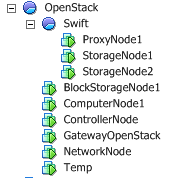
\includegraphics{openstack_tree.png}
\caption{OpenStack Nodes}
\label{overflow}
\end{figure}


\begin{figure}[ht!]
\centering
%[width=90mm]
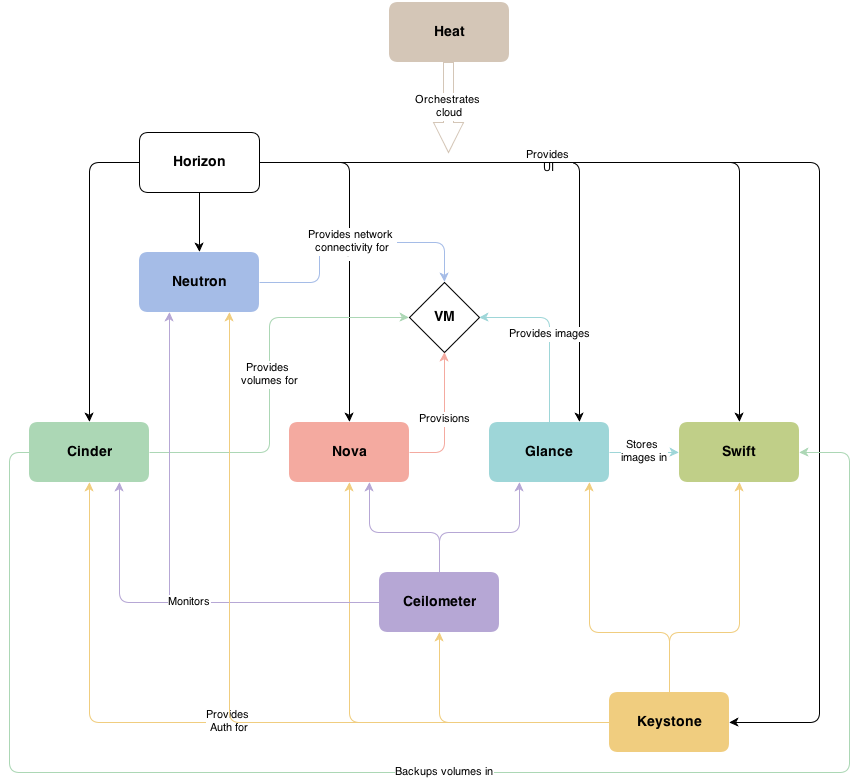
\includegraphics[width=\textwidth]{openstack_conceptual_architecture.png}
\caption{OpenStack conceptual architecture}
\label{overflow}
\end{figure}


\begin{figure}[ht!]
\centering
%[width=90mm]
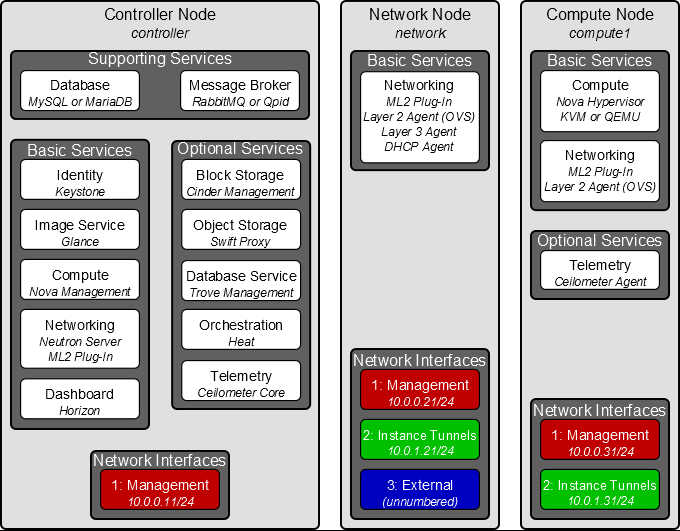
\includegraphics[width=\textwidth]{openstack_architecture.png}
\caption{OpenStack architecture}
\label{overflow}
\end{figure}

The sections just cover basic information about OpenStack. To learn more please visit official web site [5]. On the web site you can find all needed information about OpenStack, each service, installation documentation and other relevant information. One thing is needed to mention is that OpenStack is quit new project. It started in July 2010. But during passed four years it achieved big results. The next step will be attempt to make a research by using OpenStack environment. 


\subsection{Security Lab Generator based on OpenStack}
OpenStack is open source Infrastructure as a Service that provides capability to run any complex network environments. The idea of Security Lab based on OpenStack (CloudSLG) is migrating the current SLG project on the cloud. It will allow to use wide functionality of IaaS in SLG interests. It means that will not need care about how to run, configure the network, how to connect to running instance. It will allow to concentrate in solving more research questions such as analyzing user activities, finding user attack graph, reporting analytic statistics. Also, migration SLG into the cloud can be the first step of making Open Research Cloud.    





%\end{document} 